\documentclass[12pt,a4paper]{article}

\usepackage[utf8]{inputenc}
\usepackage[T1]{fontenc}
\usepackage[ngerman]{babel}
\usepackage{geometry}
\usepackage{listings}
\usepackage{xcolor}
\usepackage{hyperref}
\usepackage{amsmath}
\usepackage{booktabs}
\usepackage{caption}
\usepackage{parskip}
\usepackage{siunitx}
\usepackage{dirtree}
\usepackage{pgfplots}
\pgfplotsset{compat=1.18}
\usepackage{pgfplotstable}
\usepackage{amssymb}
\usepackage{graphicx}
\usepackage{tikz}
\usepackage{float}
\usepackage{tabularx}
\newcolumntype{R}{>{\raggedleft\arraybackslash}X}

\geometry{margin=2.5cm}

\lstdefinestyle{cuda}{
    language=C++,
    basicstyle=\ttfamily\small,
    keywordstyle=\color{blue}\bfseries,
    commentstyle=\color{gray}\itshape,
    stringstyle=\color{teal},
    numbers=left,
    numberstyle=\tiny\color{gray},
    frame=single,
    breaklines=true,
    captionpos=b,
    tabsize=4
}

\title{\textbf{Praktikumsbericht -- Projekt} \\[0.5em]
\large Canny Edge Detection auf der GPU}
\author{Matthias Stefan \and Thomas Jurczyk}
\date{\today}

\begin{document}

    \maketitle
    \tableofcontents
    \newpage

% ════════════════════════════════════════════════════════════════════════════
    \section{Voraussetzungen und Projektaufbau}
% ════════════════════════════════════════════════════════════════════════════

    \subsection{Hardware-Spezifikationen}

    \subsubsection*{System: Matthias Stefan}

    \subsubsection*{System: Thomas Jurczyk}

    \subsection{Projektstruktur}

    \subsection{Build-System und Kompilierung}

    \subsection{Messmethodologie}

    Die Performance-Messungen wurden unter nicht-isolierten Bedingungen durchgeführt. Folgende Faktoren können die Ergebnisse beeinflusst haben:

    \begin{itemize}
        \item Hintergrundprozesse liefen parallel zur Messung
        \item Thermisches Throttling durch unkontrollierte GPU-Temperatur
        \item Dynamisches Power Management der Laptop-GPU
        \item Nicht garantiert geleerte CPU- und GPU-Caches zwischen den Runs
        \item OS-Scheduling-Interrupts, insbesondere bei H$\to$D/D$\to$H Transfers
    \end{itemize}

    Die Ergebnisse sind daher als Richtwerte zu verstehen. Um Schwankungen zu minimieren, wurde jede Messung als Durchschnitt über 200 Runs ermittelt. Der erste Aufruf (Warm-up Run) wird separat ausgewiesen, da CUDA-Kontext und Page-Cache zu diesem Zeitpunkt noch nicht aufgewärmt sind. NCU-Profiling wurde mit 10 Kernel-Instanzen pro Report durchgeführt, der Warm-up Run ausgeschlossen.

    \newpage

% ════════════════════════════════════════════════════════════════════════════
    \section{Algorithmus}
% ════════════════════════════════════════════════════════════════════════════

    \subsection{Überblick}

    Der Canny-Algorithmus ist ein mehrstufiges Verfahren zur Kantendetektion in
    Graustufenbildern. Canny definiert drei Kriterien für einen optimalen
    Kantendetektor: gute Detektion, präzise Lokalisierung sowie exakt eine Antwort
    pro Kante -- jede Kante soll auf eine Breite von einem Pixel supprimiert werden
    \cite[S.~680]{canny1986}. Die Verarbeitung erfolgt in vier aufeinanderfolgenden
    Schritten, wobei der Output jedes Schritts als Input des nächsten dient
    (siehe Abbildung~\ref{fig:pipeline}). Die einzelnen Schritte werden in den
    kommenden Abschnitten näher erläutert.

    \begin{figure}[h]
        \centering
        \resizebox{\textwidth}{!}{
            \begin{tikzpicture}[
                box/.style={rectangle, draw, rounded corners, minimum width=2.8cm,
                minimum height=1cm, align=center, font=\small},
                arrow/.style={->, thick}
            ]
        \node[box, fill=gray!20]   (input)  at (0,0)    {Eingabebild};
        \node[box, fill=blue!15]   (blur)   at (3.5,0)  {Schritt 1\\Gaussian Blur};
        \node[box, fill=teal!15]   (sobel)  at (7,0)    {Schritt 2\\Gradient (Sobel)};
        \node[box, fill=orange!15] (nms)    at (10.5,0) {Schritt 3\\Non-Max. Supp.};
        \node[box, fill=red!15]    (hyst)   at (14,0)   {Schritt 4\\Hysteresis};
        \node[box, fill=gray!20]   (output) at (17.5,0) {Kantenbild};

        \draw[arrow] (input)  -- (blur);
        \draw[arrow] (blur)   -- (sobel);
        \draw[arrow] (sobel)  -- (nms);
        \draw[arrow] (nms)    -- (hyst);
        \draw[arrow] (hyst)   -- (output);
            \end{tikzpicture}
        }
        \caption{Canny Edge Detection Pipeline}
        \label{fig:pipeline}
    \end{figure}

    \subsection{Details}

    \subsubsection{Schritt 1: Gaussian Blur}

    Um einen mathematisch optimalen Kantendetektor herzuleiten, trifft Canny
    eine Annahme über das Rauschen im Bild: \textit{,,We will assume that the
    image consists of the edge and additive white Gaussian noise``}
    \cite[S.~680]{canny1986}. Da dieses Rauschen fälschlicherweise als Kante
    detektiert werden kann, muss das Bild zunächst geglättet werden. Canny
    zeigt, dass der optimale Filter für dieses Rauschmodell durch die erste
    Ableitung einer Gaußfunktion approximiert werden kann
    \cite[S.~687]{canny1986}:

    \begin{equation}
        \label{eq:gaussian}
        G(x) = \exp\left(-\frac{x^2}{2\sigma^2}\right)
    \end{equation}

    Der Parameter $\sigma$ kontrolliert die Stärke der Glättung. Zwischen
    Rauschunterdrückung und Lokalisierungsgenauigkeit besteht jedoch ein
    grundlegender Zielkonflikt -- Canny bezeichnet dies als
    \textit{,,uncertainty principle``} zwischen Detektion und Lokalisierung
    \cite[S.~684]{canny1986}.

    \subsubsection{Schritt 2: Gradient Berechnung (Sobel)}

    \subsubsection{Schritt 3: Non-Maximum Suppression}

    Schritt~2 liefert für jeden Pixel einen Gradientenbetrag, der die lokale
    Kantenstärke beschreibt, die resultierenden Kanten sind dabei an vielen
    Stellen breiter als ein Pixel. Canny fordert jedoch präzise Lokalisierung:
    \textit{,,The points marked as edge points by the operator should be as close
    as possible to the center of the true edge``} \cite[S.~680]{canny1986}.
    Non-Maximum Suppression reduziert diese breite Gradientenantwort auf eine
    Breite von einem Pixel, indem entlang der Gradientenrichtung nur das lokale
    Maximum erhalten bleibt.

    Formal lässt sich der gesuchte Kantenpunkt als Nullstelle der zweiten
    Richtungsableitung des geglätteten Bildes beschreiben:

    \begin{equation}
        \label{eq:nms_condition}
        \frac{\partial^2}{\partial n^2} (G * I) = 0
    \end{equation}

    wobei $n$ die Richtung des Gradienten bezeichnet und $G * I$ das geglättete
    Bild \cite[S.~691]{canny1986}. Die Nullstelle der zweiten Ableitung markiert
    exakt den Punkt, an dem die erste Ableitung, die Gradientenstärke entlang
    $n$, ihr lokales Maximum besitzt. Da die Kantenrichtung $n$ nicht vorab
    bekannt ist, wird sie aus der geglätteten Gradientenrichtung geschätzt
    \cite[Gl.~46, S.~691]{canny1986}:

    \begin{equation}
        \label{eq:edge_direction}
        n = \frac{\nabla(G * I)}{|\nabla(G * I)|}
    \end{equation}

    In der diskreten Implementierung wird Gleichung~\ref{eq:nms_condition}
    approximiert, indem die Gradientenmagnitude $|\nabla(G * I)|$ jedes Pixels
    mit den beiden direkten Nachbarn entlang der auf vier Klassen
    ($0^\circ$/$45^\circ$/$90^\circ$/$135^\circ$) quantisierten Gradientenrichtung verglichen wird. Ein
    Pixel überlebt die Suppression genau dann, wenn seine Magnitude größer oder
    gleich beiden Nachbarn ist, andernfalls wird er auf null gesetzt.

    \subsubsection{Schritt 4: Hysteresis Thresholding}

    \newpage

% ════════════════════════════════════════════════════════════════════════════
    \section{Implementierung}
% ════════════════════════════════════════════════════════════════════════════

    \subsection{Schritt 1: Gaussian Blur}

    \subsubsection{Naive Implementierung}

    Die Gaußgewichte werden zunächst auf der CPU als zweidimensionales Raster der
    Größe $(2 \cdot \texttt{BLUR\_RADIUS} + 1)^2$ vorberechnet und normalisiert,
    sodass ihre Summe~1 ergibt und die Bildhelligkeit erhalten bleibt
    (Gleichung~\ref{eq:gaussian}). Das Gewichtsraster wird einmalig vor dem
    Kernelaufruf per \texttt{cudaMemcpy} auf die GPU übertragen und steht dort
    allen Threads als Read-only-Buffer im globalen Speicher zur Verfügung.
    Das resultierende $3 \times 3$ Gewichtsraster für $\sigma = 1.0$ ist in
    Abbildung~\ref{fig:gaussian_example} dargestellt.

    \begin{figure}[H]
        \centering
        \begin{tikzpicture}[
            pixel/.style={rectangle, draw, minimum size=1.3cm, align=center, font=\small, inner sep=2pt},
            k_low/.style={pixel,  fill=red!20},
            k_mid/.style={pixel,  fill=red!35},
            k_high/.style={pixel, fill=red!55}
        ]

    \node[k_low]  at (0,0)      {0.0894};
    \node[k_mid]  at (1.4,0)    {0.1201};
    \node[k_low]  at (2.8,0)    {0.0894};
    \node[k_mid]  at (0,-1.4)   {0.1201};
    \node[k_high] at (1.4,-1.4) {0.1615};
    \node[k_mid]  at (2.8,-1.4) {0.1201};
    \node[k_low]  at (0,-2.8)   {0.0894};
    \node[k_mid]  at (1.4,-2.8) {0.1201};
    \node[k_low]  at (2.8,-2.8) {0.0894};

    \node[font=\Large] at (4.0,-1.4) {$\times$};

    \node[pixel, fill=black!90, text=white] at (5.3,0)    {L10};
    \node[pixel, fill=black!70, text=white] at (6.7,0)    {L20};
    \node[pixel, fill=black!50, text=white] at (8.1,0)    {L30};
    \node[pixel, fill=black!45, text=white] at (5.3,-1.4) {L50};
    \node[pixel, fill=black!50, text=white] at (6.7,-1.4) {L48};
    \node[pixel, fill=black!90, text=white] at (8.1,-1.4) {L10};
    \node[pixel, fill=black!10]             at (5.3,-2.8) {L90};
    \node[pixel, fill=black!60, text=white] at (6.7,-2.8) {L30};
    \node[pixel, fill=black!70, text=white] at (8.1,-2.8) {L20};

    \node[font=\Large] at (9.4,-1.4) {$=$};

    \node[pixel, fill=black!55, text=white] at (10.7,-1.4) {L34};

        \end{tikzpicture}
        \caption{Gaussian Blur, gewichteter Mittelwert am Beispielpixel L48 $\rightarrow$ L34}
        \label{fig:gaussian_example}
    \end{figure}

    Im CUDA-Kernel \texttt{gaussian\_filter()} ist jeder Thread für genau einen
    Ausgabepixel zuständig. Die Thread-Position ergibt sich aus \texttt{blockIdx}
    und \texttt{threadIdx} (Listing~\ref{lst:gaussian_kernel}, Zeile~1--2), Threads
    außerhalb der Bildgrenzen werden sofort verworfen (Zeile~3). Jeder Thread
    iteriert anschließend über alle $(2r+1)^2$ Nachbarpixel, liest jeden Wert
    direkt aus dem globalen Speicher und akkumuliert die gewichtete Summe
    (Zeile~5--10). Pixel außerhalb der Bildgrenzen werden mit~0 aufgefüllt
    (Zero-Padding). Das Ergebnis wird in den Ausgabepuffer geschrieben (Zeile~12).

    \begin{lstlisting}[style=cuda, basicstyle=\ttfamily\scriptsize,
        caption={Pseudocode, gaussian\_filter Kernel (naive)},
        label={lst:gaussian_kernel}, numbers=left]
x = blockIdx.x * blockDim.x + threadIdx.x
y = blockIdx.y * blockDim.y + threadIdx.y
if (x, y) ausserhalb des Bildes: return

color = 0.0
for j = -radius to +radius:
    for i = -radius to +radius:
        if (x+i, y+j) innerhalb des Bildes:
            pixel = src_buffer[(y+j) * width + (x+i)]
        color += pixel * weights[(j+r) * blur_size + (i+r)]

out_buffer[y * width + x] = color
    \end{lstlisting}

    Das NCU-Profiling zeigt, dass 47\,\% aller Global Memory Zugriffe uncoalesced
    sind, da benachbarte Threads in y-Richtung auf Adressen mit Abstand
    \texttt{width} zugreifen. Dies motiviert die Shared Memory Optimierung in
    Abschnitt~\ref{sec:shared_memory_gaussian}. Das Ergebnis der Filterung ist in
    Abbildung~\ref{fig:gaussian_result} dargestellt.

    \begin{figure}[H]
        \centering
        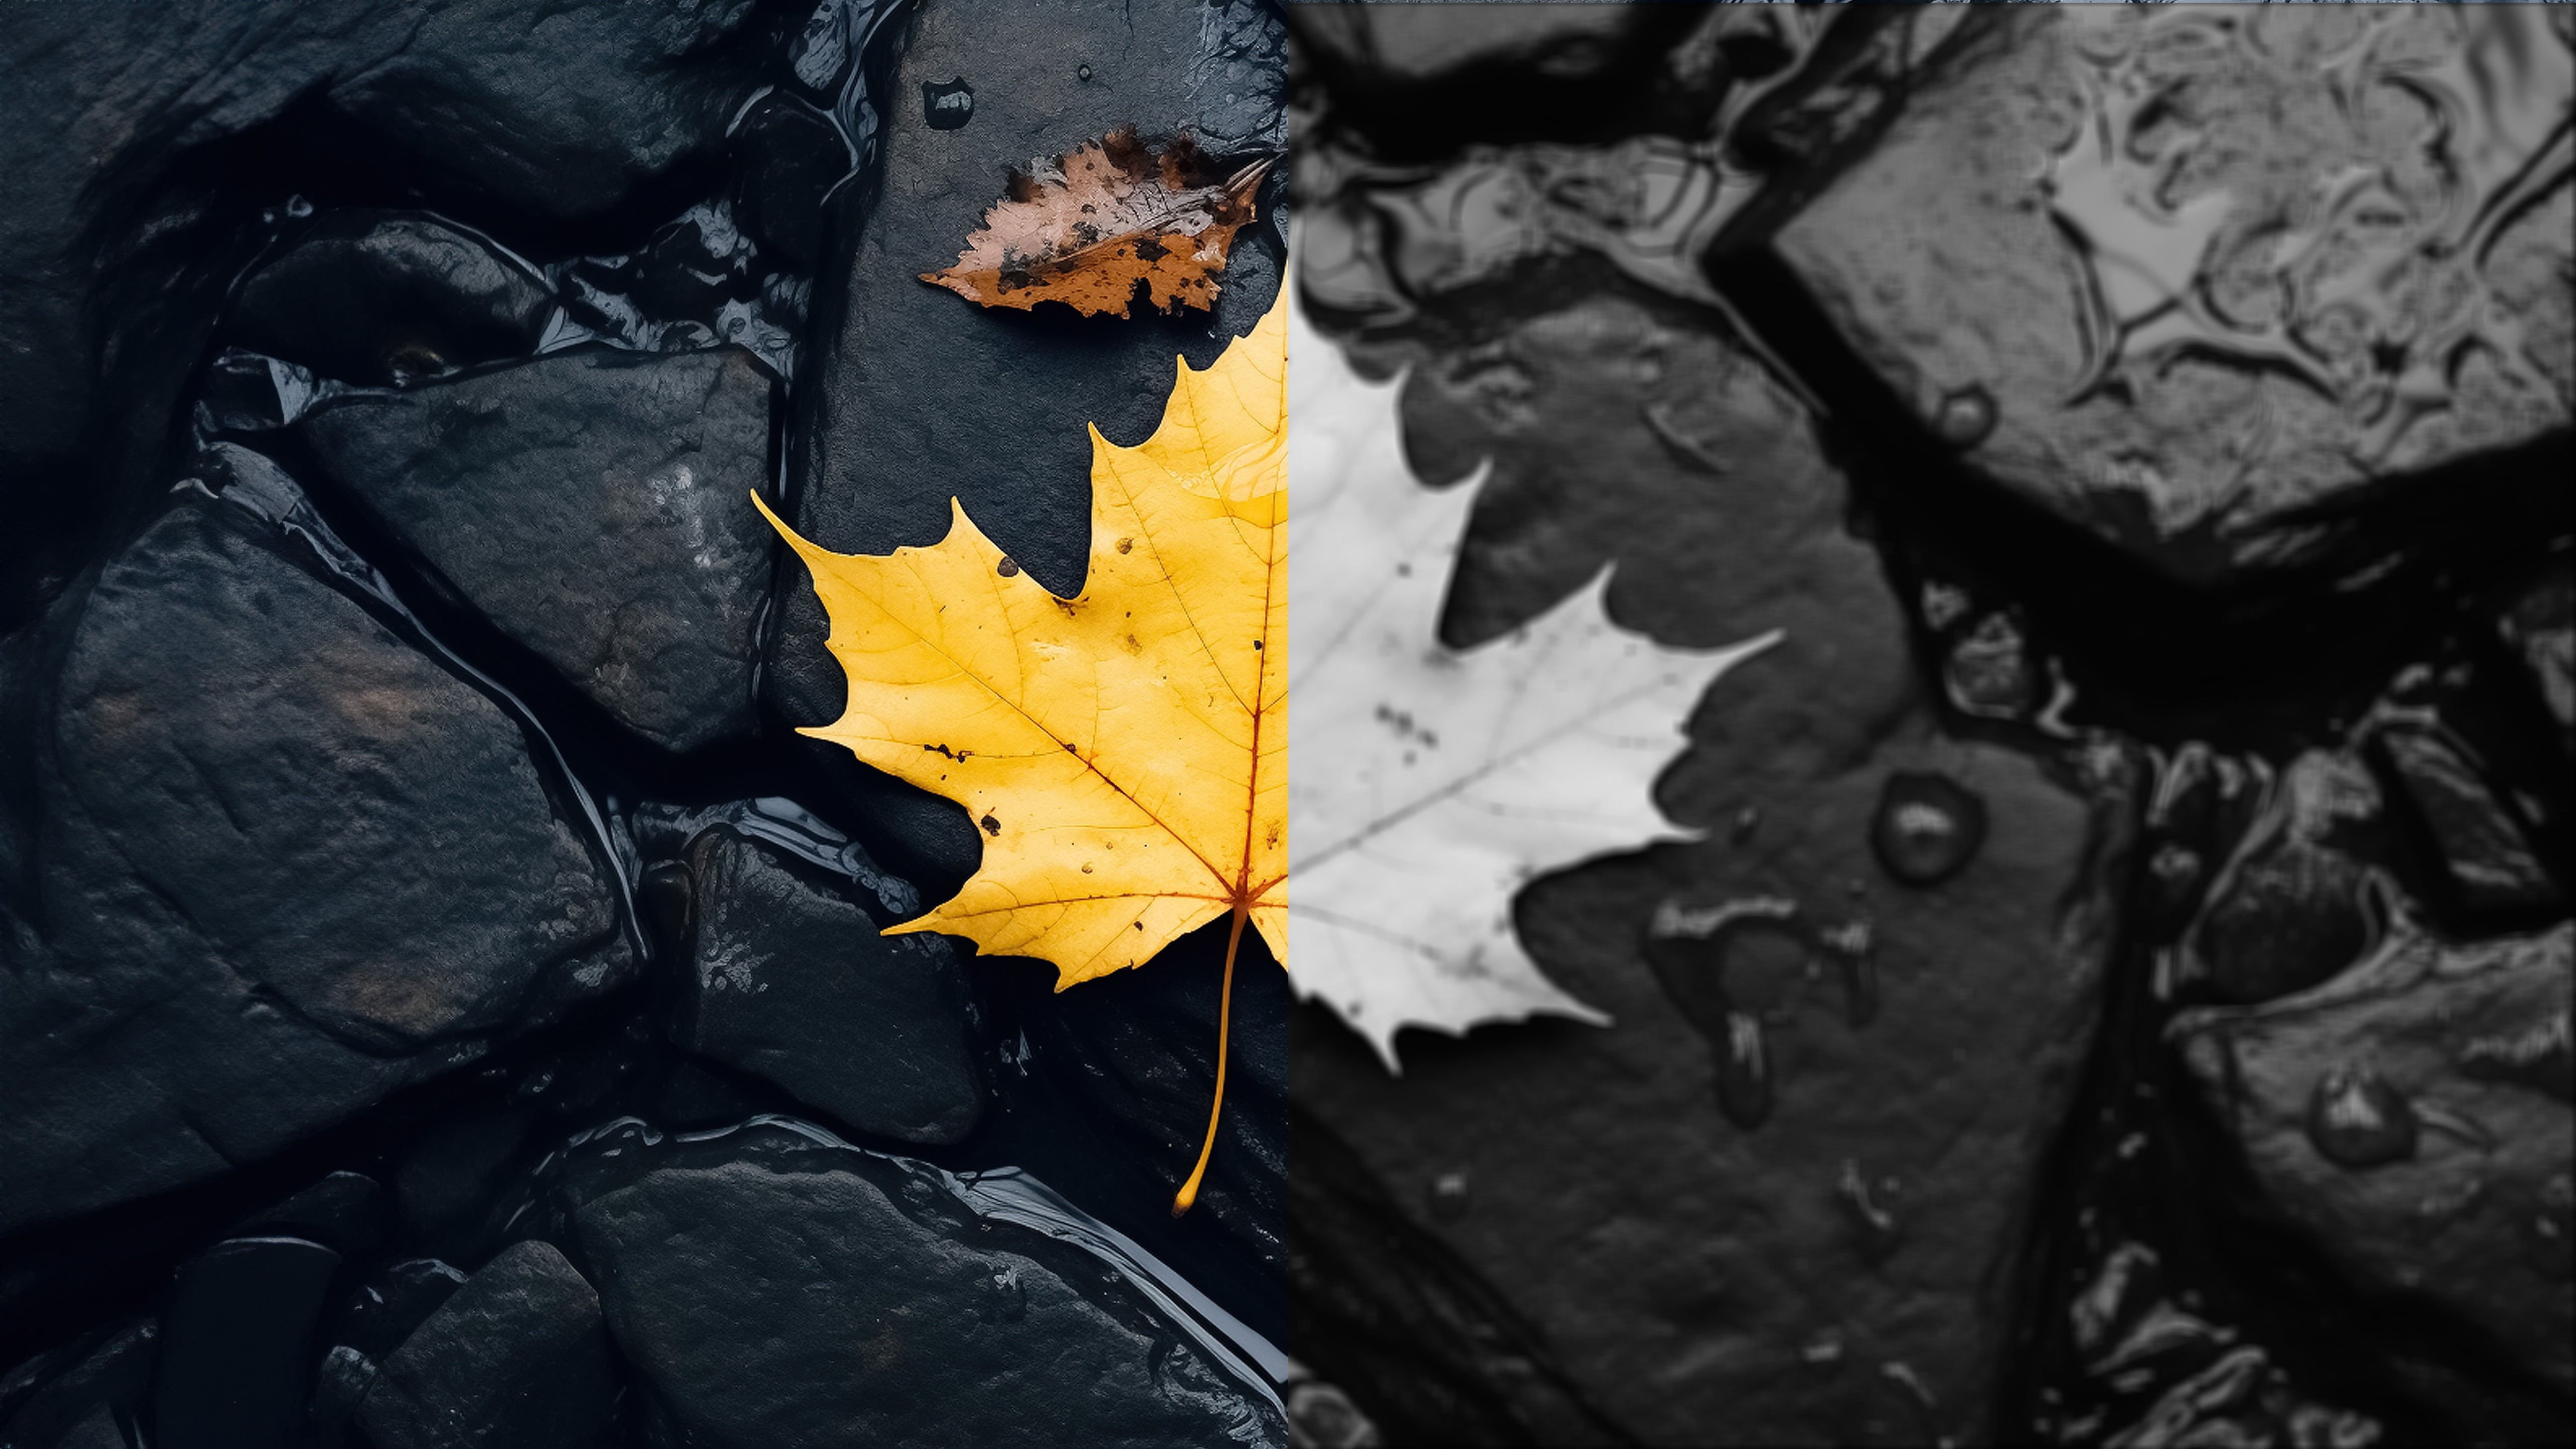
\includegraphics[width=0.7\textwidth]{../assets/maple-leaf-black-5120x2880-cmp-original-gaussian.jpg}
        \caption{Vergleich Original (links) vs.\ Gaussian Blur (rechts,
            $\sigma = 25$, \texttt{BLUR\_RADIUS}$= 12$). Die Parameter wurden
            bewusst extrem gewählt, um den Effekt deutlicher sichtbar zu machen,
            in der Pipeline wird ein deutlich sanfterer Filter verwendet.}
        \label{fig:gaussian_result}
    \end{figure}

    \subsubsection{Shared Memory Optimierung}
    \label{sec:shared_memory_gaussian}

    Der zentrale Engpass der naiven Implementierung sind die uncoalesced Global
    Memory Zugriffe: bei einem Kernel der Größe $(2r+1)^2$ liest jeder Thread
    bis zu $(2r+1)^2$ Pixel aus dem DRAM, wobei Pixel die von mehreren
    Threads benötigt werden redundant geladen werden. Horvath et al.\ adressieren
    dieses Problem durch Shared Memory Tiling, bei dem Threads eines Blocks
    kooperativ eine Bildkachel in den schnellen On-Chip Speicher laden, bevor die
    eigentliche Faltung beginnt \cite[S.~2]{horvath2023}.

    Die Kachel hat die Größe $(\texttt{BLOCK\_SIZE} + 2 \cdot
    \texttt{BLUR\_RADIUS})^2$ und enthält neben den eigentlichen Ausgabepixeln
    des Blocks auch den sogenannten Halo-Rand. Da die Kachel größer ist als der
    Block selbst, lädt jeder Thread mittels eines Stride-Loops einen oder mehrere
    Pixel in den Shared Memory. Nach dem Laden wird \texttt{\_\_syncthreads()}
    aufgerufen, um sicherzustellen, dass alle Threads ihre Pixel geschrieben haben
    bevor die Faltung beginnt. Die Gaußgewichte werden zusätzlich in
    \texttt{\_\_constant\_\_} Memory ausgelagert, da alle Threads exakt dieselben
    Gewichte lesen und \texttt{\_\_constant\_\_} Memory für uniforme Zugriffe
    hardwareseitig gecacht wird.

    Die drei wesentlichen Änderungen gegenüber der naiven Implementierung sind:

    \begin{itemize}
        \item \texttt{\_\_shared\_\_ uint8\_t tile[tile\_size * tile\_size]},
        eine kooperativ geladene Bildkachel inklusive Halo-Rand der Breite
        \texttt{BLUR\_RADIUS}
        \item \texttt{\_\_syncthreads()}, Synchronisationsbarriere nach dem
        kooperativen Laden
        \item \texttt{\_\_constant\_\_ float device\_weights[...]},
        Gaußgewichte in Constant Memory, Upload per \texttt{cudaMemcpyToSymbol()}
    \end{itemize}

    Abbildung~\ref{fig:gaussian_ncu} zeigt, dass der Speedup stark vom
    \texttt{BLUR\_RADIUS} abhängt. Bei $r=2$ überwiegt der \texttt{\_\_syncthreads()}-Overhead, die Kernel-Laufzeit
    sinkt nur marginal von 1.67\,ms auf 0.99\,ms bei nahezu identischem SM Throughput
    (68.31\,\% vs.\ 66.25\,\%). Bei $r=9$ kehrt sich das Verhältnis um: die
    $(2 \cdot 9 + 1)^2 = 361$ Operationen pro Pixel machen den redundanten
    DRAM-Traffic zum dominanten Faktor, die Kernel-Laufzeit sinkt von 22.67\,ms
    auf 7.54\,ms ($3.0\times$ Speedup), der SM Throughput steigt von 64.66\,\%
    auf 91.50\,\%. Die vollständigen Messdaten sind in Anhang~A (S.~\pageref{app:gaussian_rohdaten}) aufgeführt.

    \begin{figure}[H]
        \centering
        \begin{minipage}{0.48\textwidth}
            \begin{tikzpicture}
                \begin{axis}[
                    ybar,
                    bar width=10pt,
                    title={SM Throughput (\%)},
                title style={font=\footnotesize},
                xtick={1,2},
                xticklabels={$r{=}2$, $r{=}9$},
                xticklabel style={font=\small},
                width=\textwidth, height=6cm,
                ymin=0, ymax=115,
                enlarge x limits=0.4,
                legend style={at={(0.5,-0.25)}, anchor=north, legend columns=3, font=\tiny},
                nodes near coords,
                nodes near coords style={font=\tiny, rotate=90, anchor=west},
                ]
                    \addplot[fill={rgb,255:red,70;green,130;blue,200}]  coordinates {(1,68.31) (2,64.66)};
                    \addplot[fill={rgb,255:red,240;green,160;blue,50}]  coordinates {(1,66.25) (2,91.50)};
                    \addplot[fill={rgb,255:red,100;green,190;blue,120}] coordinates {(1,66.54) (2,91.46)};
                    \legend{naive, shared, pinned}
                \end{axis}
            \end{tikzpicture}
        \end{minipage}
        \hfill
        \begin{minipage}{0.48\textwidth}
            \begin{tikzpicture}
                \begin{axis}[
                    ybar,
                    bar width=10pt,
                    title={Kernel Duration (ms)},
                title style={font=\footnotesize},
                xtick={1,2},
                xticklabels={$r{=}2$, $r{=}9$},
                xticklabel style={font=\small},
                width=\textwidth, height=6cm,
                ymin=0, ymax=27,
                enlarge x limits=0.4,
                legend style={at={(0.5,-0.25)}, anchor=north, legend columns=3, font=\tiny},
                nodes near coords,
                nodes near coords style={font=\tiny, rotate=90, anchor=west},
                ]
                    \addplot[fill={rgb,255:red,70;green,130;blue,200}]  coordinates {(1,1.67) (2,22.67)};
                    \addplot[fill={rgb,255:red,240;green,160;blue,50}]  coordinates {(1,0.99) (2, 7.54)};
                    \addplot[fill={rgb,255:red,100;green,190;blue,120}] coordinates {(1,0.99) (2, 7.33)};
                    \legend{naive, shared, pinned}
                \end{axis}
            \end{tikzpicture}
        \end{minipage}
        \caption{NCU-Profiling, Vergleich naive/shared/pinned bei $r{=}2$ und $r{=}9$ (200 Runs Avg).}
        \label{fig:gaussian_ncu}
    \end{figure}

    \subsubsection{Pinned Memory Optimierung}
    \label{sec:pinned_memory_gaussian}

    Pinned Memory (Page-locked Memory) ist Host-seitiger Speicher, der vom
    Betriebssystem nicht ausgelagert werden kann, wodurch direkte DMA-Transfers
    ohne zwischengeschalteten CPU-Cache möglich sind. Die Änderung gegenüber
    der Shared Memory Implementierung beschränkt sich ausschließlich auf die
    Host-seitige Allokation (\texttt{cudaMallocHost()} statt \texttt{malloc()}),
    der Kernel bleibt identisch, was die NCU-Messungen bestätigen: Compute
    Throughput und Occupancy sind bei $r=9$ mit 91.46\,\% bzw.\ 94.83\,\%
    praktisch identisch zur Shared Memory Variante (91.50\,\% bzw.\ 94.84\,\%).
    Der Vorteil zeigt sich ausschließlich im D$\to$H Transfer, der bei $r=9$
    von 2.04\,ms auf 1.37\,ms sinkt, und im Gesamttiming von 11.95\,ms auf
    10.75\,ms. Die vollständigen Messdaten sind im Anhang~A (S.~\pageref{app:gaussian_rohdaten}) aufgeführt.

    \subsubsection{Warp-Level Optimierung - Evaluation}

    Als vierte Optimierungsstufe wurden Warp-Level Intrinsics (\texttt{\_\_shfl\_sync()})
    evaluiert. Diese ermöglichen den direkten Datenaustausch zwischen Threads
    innerhalb eines Warps ohne Shared Memory und ohne \texttt{\_\_syncthreads()}.

    Für 2D-Stencil-Operationen wie den Gaussian Blur ist dieser Ansatz jedoch
    nicht geeignet, da \texttt{\_\_shfl\_sync()} primär für 1D-Reduktionen
    konzipiert ist und bei zweidimensionalen Nachbarschaftszugriffen keinen
    strukturellen Vorteil bietet. Yadav et al.\ bestätigen dies: in ihren
    Messungen erreicht die Warp-Variante 79.29\,\% Compute/Memory Throughput,
    während Shared Memory 83.33\,\% erzielt \cite{yadav2025}. Eine eigene
    Implementierung wurde daher nicht vorgenommen.


    \subsection{Schritt 2: Gradient Berechnung (Sobel)}

    \subsection{Schritt 3: Non-Maximum Suppression}

    Die Non-Maximum Suppression wird im CUDA-Kernel
    \texttt{non\_maximum\_suppression()} umgesetzt. Jeder Thread ist dabei für
    genau einen Pixel zuständig, die Thread-Position ergibt sich wie in
    Schritt~1 und~2 aus \texttt{blockIdx} und \texttt{threadIdx}. Als Input
    erhält der Kernel den Gradientenbetrag (\texttt{magnitude\_buffer}) sowie
    die Gradientenrichtung in Radiant (\texttt{direction\_buffer}) aus
    Schritt~2.

    Zunächst wird die Gradientenrichtung von Radiant in Grad umgerechnet und
    auf den Bereich $[0^\circ, 180^\circ)$ gefaltet, da eine Kante keine
    Orientierung besitzt, eine Kante bei $170^\circ$ und eine bei $-10^\circ$
    beschreiben dieselbe Achse. Anschließend wird die Richtung auf eine von
    vier Klassen quantisiert, die den vier möglichen Achsen im diskreten
    Pixelraster entsprechen (siehe Abbildung~\ref{fig:nms_directions}).

    Je nach Richtungsklasse werden die Offsets $(dx, dy)$ zum Nachbarpixel
    bestimmt (Listing~\ref{lst:nms_kernel}, Zeile~18--22). Der Pixel überlebt
    die Suppression genau dann, wenn seine Magnitude größer oder gleich beiden
    Nachbarn entlang dieser Achse ist (Zeile~24--26), andernfalls wird er auf
    null gesetzt:

    \begin{lstlisting}[style=cuda, basicstyle=\ttfamily\scriptsize,
        caption={non\_maximum\_suppression Kernel},
        label={lst:nms_kernel}, numbers=left]
__global__ void non_maximum_suppression(
    const uint8_t* magnitude_buffer,
    const float* direction_buffer,
    const int32_t width,
    const int32_t height,
    uint8_t* out_nms_buffer)
{
    const auto x = static_cast<int32_t>(blockIdx.x * blockDim.x + threadIdx.x);
    const auto y = static_cast<int32_t>(blockIdx.y * blockDim.y + threadIdx.y);
    if (x >= width || y >= height)
        return;

    const uint8_t magnitude = magnitude_buffer[y * width + x];
    const float direction = direction_buffer[y * width + x];

    float deg = direction * (180.0f / CUDART_PI_F);
    deg = fmodf(deg + 180.0f, 180.0f);

    int32_t dx, dy;
    if (deg < 22.5f)       { dx = 1; dy =  0; }
    else if (deg < 67.5f)  { dx = 1; dy = -1; }
    else if (deg < 112.5f) { dx = 0; dy =  1; }
    else if (deg < 157.5f) { dx = 1; dy =  1; }
    else                   { dx = 1; dy =  0; }

    const uint8_t neighbor_a =
        sample_clamped(magnitude_buffer, width, height, x + dx, y + dy);
    const uint8_t neighbor_b =
        sample_clamped(magnitude_buffer, width, height, x - dx, y - dy);

    out_nms_buffer[y * width + x] =
        (magnitude >= neighbor_a && magnitude >= neighbor_b) ? magnitude : 0;
}
    \end{lstlisting}

    \begin{figure}[H]
        \centering
        \begin{tikzpicture}[
            pixel/.style={rectangle, draw, minimum size=1.1cm, align=center,
            font=\small, inner sep=2pt, fill=gray!15},
            center/.style={rectangle, draw, minimum size=1.1cm, align=center,
            font=\small\bfseries, inner sep=2pt, fill=orange!30},
            n_violet/.style={rectangle, draw, minimum size=1.1cm, align=center,
            font=\small, inner sep=2pt, fill=violet!25},
        ]

            %% Panel 1: Richtung
            \foreach \col in {0,1,2} {
                \foreach \row in {0,1,2} {
                    \node[pixel] at (\col*1.3, -\row*1.3) {};
                }
            }
            \node[center] at (1.3,-1.3) {};
            \draw[->, line width=2pt, violet!80] (1.3,-1.3) -- (2.5,-2.0);
            \node[font=\small] at (1.3,-3.9) {Richtung};
            \node[font=\tiny, text=gray] at (1.3,-4.3) {(beliebiger Winkel)};

            %% Pfeil
            \draw[->, thick] (3.4,-1.3) -- (4.2,-1.3);

            %% Panel 2: 4 Richtungen
            \coordinate (O) at (6.0,-1.3);
            \draw[->, very thick, black]         (O) -- ++(1.2, 0)       node[right, font=\small] {$0^\circ$};
            \draw[->, line width=2pt, violet!80] (O) -- ++(0.85,-0.85)   node[right, font=\small] {$45^\circ$};
            \draw[->, very thick, black]         (O) -- ++(0,-1.2)       node[below, font=\small] {$90^\circ$};
            \draw[->, very thick, black]         (O) -- ++(-0.85,-0.85)  node[left,  font=\small] {$135^\circ$};
            \node[font=\small, align=center] at (6.0,-3.9) {eine von vier\\Richtungen};

            %% Pfeil
            \draw[->, thick] (8.0,-1.3) -- (8.8,-1.3);

            %% Panel 3: Vergleich
            \foreach \col in {0,1,2} {
                \foreach \row in {0,1,2} {
                    \node[pixel] at (9.2+\col*1.3, -\row*1.3) {};
                }
            }
            \node[center]   at (9.2+1.3, -1.3) {};
            \node[n_violet] at (9.2+2.6, -2.6) {};   % SE
            \node[n_violet] at (9.2+0,    0)   {};   % NW
            \node[font=\small] at (9.2+1.3,-3.9) {Vergleich};

        \end{tikzpicture}
        \caption{Non-Maximum Suppression: Die Gradientenrichtung wird auf eine von
        vier Achsen quantisiert ($0^\circ$, $45^\circ$, $90^\circ$, $135^\circ$).
        Anschließend wird der Pixel mit den beiden farbig markierten Nachbarn entlang
        der gewählten Achse verglichen.}
        \label{fig:nms_directions}
    \end{figure}

    Das Ergebnis der Non-Maximum Suppression ist in
    Abbildung~\ref{fig:nms_result} dargestellt. Im Vergleich zur
    Gradientenmagnitude aus Schritt~2 sind die Kanten auf eine Breite von
    einem Pixel reduziert.

    \begin{figure}[H]
        \centering
        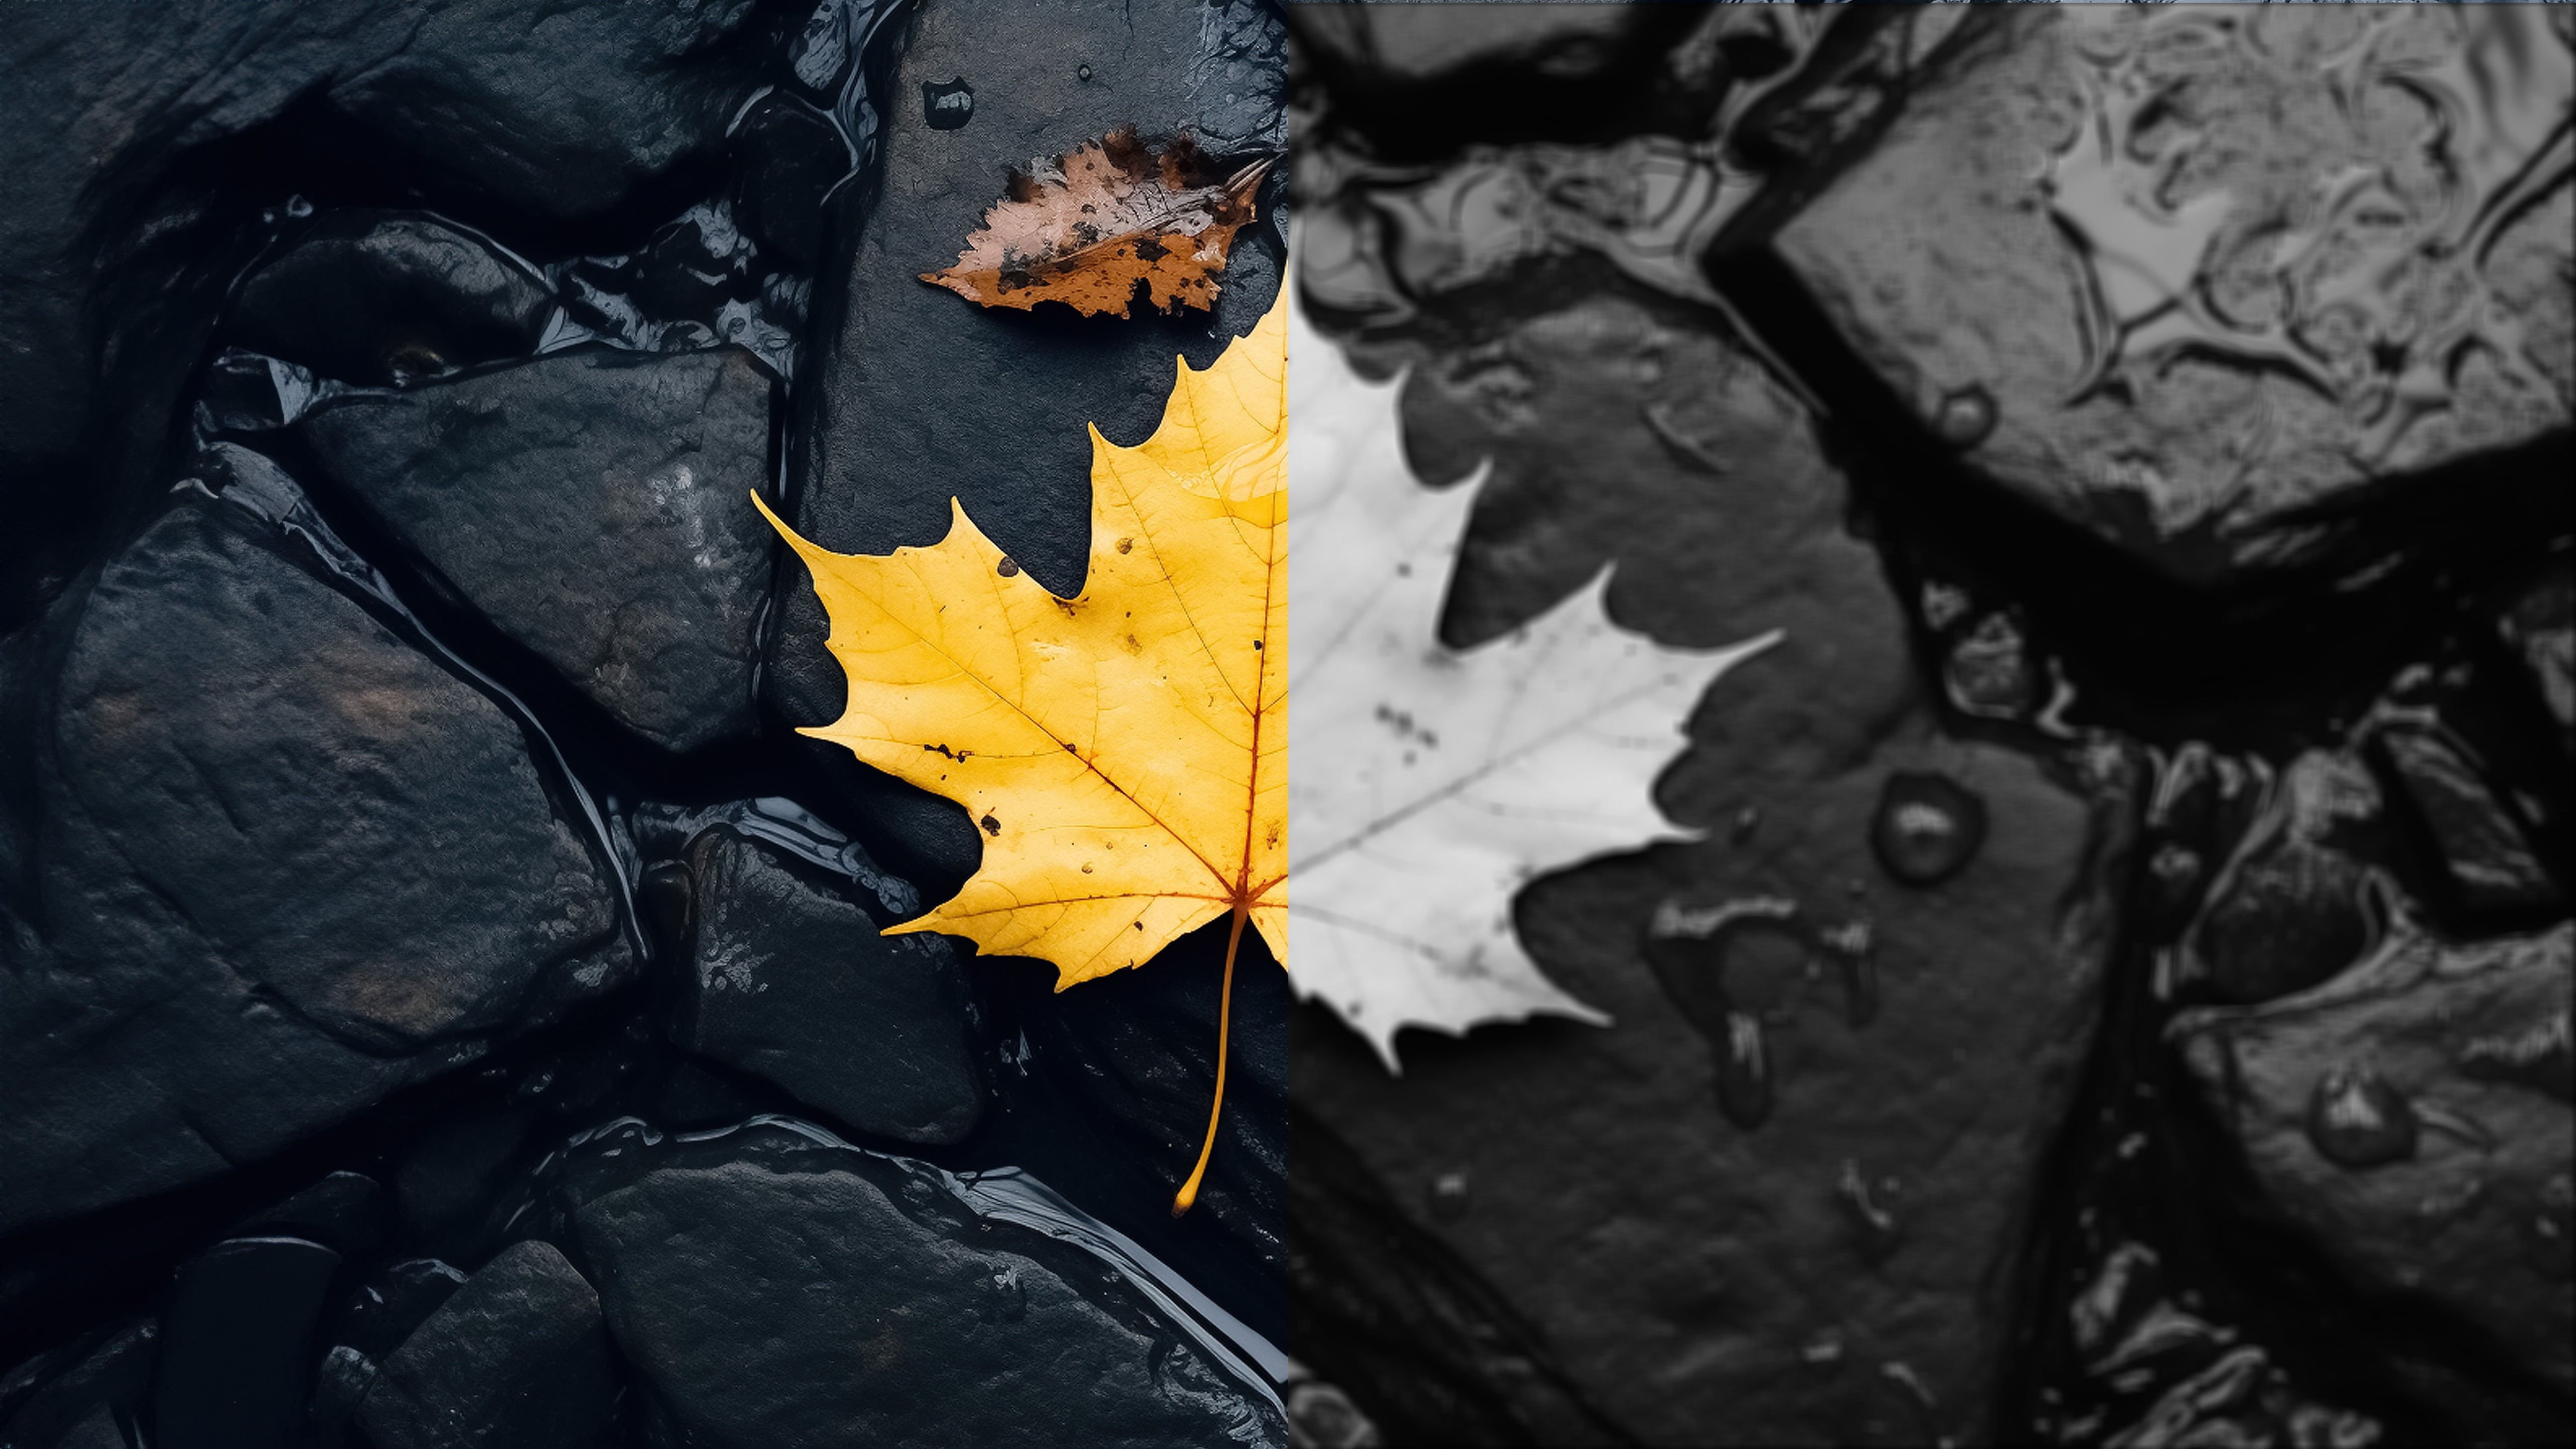
\includegraphics[width=0.7\textwidth]{../assets/maple-leaf-black-5120x2880-cmp-original-gaussian.jpg}
        \caption{Vergleich Gradientenmagnitude (links) vs.\ Non-Maximum
        Suppression (rechts), die breite Gradientenantwort wird auf
        eine Breite von einem Pixel reduziert. (Placeholder -- wird ersetzt)}
        \label{fig:nms_result}
    \end{figure}


    \subsection{Schritt 4: Hysteresis Thresholding}



    \newpage

% ════════════════════════════════════════════════════════════════════════════
    \section{Ergebnisse und Analyse}
% ════════════════════════════════════════════════════════════════════════════

    \subsection{Korrektheit}

    \subsection{Performance-Messungen}

    \subsection{Analyse}

    \newpage

% ════════════════════════════════════════════════════════════════════════════
    \section{Fazit}
% ════════════════════════════════════════════════════════════════════════════

    \newpage

    \bibliographystyle{plain}
    \bibliography{references}

    \newpage

% ════════════════════════════════════════════════════════════════════════════
    \section*{Anhang}
    \addcontentsline{toc}{section}{Anhang}
% ════════════════════════════════════════════════════════════════════════════

    \phantomsection
    \subsection*{A: Performance-Rohdaten Gaussian Blur}
    \label{app:gaussian_rohdaten}

    \begin{table}[H]
        \begin{tabularx}{\textwidth}{lRRR}
\toprule
Metrik & naive & shared & pinned \\
\midrule
\multicolumn{4}{l}{\textit{Warm-up Run}} \\
H$\to$D [ms]  &  3.062 &  5.660 &  2.709 \\
Kernel [ms]   &  2.606 &  1.697 &  1.688 \\
D$\to$H [ms]  &  7.631 &  7.020 &  2.502 \\
Total [ms]    & 13.299 & 14.377 &  6.899 \\
\midrule
\multicolumn{4}{l}{\textit{200 Runs Avg}} \\
H$\to$D [ms]  &  3.548 &  3.475 &  3.135 \\
Kernel [ms]   &  1.669 &  0.990 &  0.987 \\
D$\to$H [ms]  &  3.068 &  3.001 &  1.740 \\
Total [ms]    &  8.286 &  7.466 &  5.862 \\
\bottomrule
        \end{tabularx}
        \caption{cudaEvent-Messungen, BLUR\_RADIUS = 2}
    \end{table}

    \begin{table}[H]
        \begin{tabularx}{\textwidth}{lRRR}
\toprule
Metrik (NCU, 10 Runs Avg) & naive & shared & pinned \\
\midrule
Compute (SM) Throughput [\%]       & 68.31 & 66.25 & 66.54 \\
Memory Throughput [\%]             & 61.10 & 66.25 & 66.54 \\
DRAM Throughput [\%]               &  5.81 &  8.42 &  7.60 \\
Achieved Occupancy [\%]            & 76.50 & 92.67 & 92.65 \\
Warp Cycles Per Issued Instruction &  8.79 & 16.46 & 16.33 \\
L1/TEX Hit Rate [\%]               & 92.94 & 27.32 & 27.29 \\
L2 Hit Rate [\%]                   & 87.75 & 88.17 & 89.12 \\
\bottomrule
        \end{tabularx}
        \caption{NCU-Profiling, BLUR\_RADIUS = 2}
    \end{table}

    \begin{table}[H]
        \begin{tabularx}{\textwidth}{lRRR}
\toprule
Metrik & naive & shared & pinned \\
\midrule
\multicolumn{4}{l}{\textit{Warm-up Run}} \\
H$\to$D [ms]  &  2.589 &  1.757 &  1.781 \\
Kernel [ms]   & 35.700 & 12.575 & 13.182 \\
D$\to$H [ms]  &  6.035 &  6.183 &  1.836 \\
Total [ms]    & 44.324 & 20.515 & 16.799 \\
\midrule
\multicolumn{4}{l}{\textit{200 Runs Avg}} \\
H$\to$D [ms]  &  2.512 &  2.375 &  2.057 \\
Kernel [ms]   & 22.669 &  7.537 &  7.325 \\
D$\to$H [ms]  &  2.142 &  2.036 &  1.366 \\
Total [ms]    & 27.308 & 11.948 & 10.747 \\
\bottomrule
        \end{tabularx}
        \caption{cudaEvent-Messungen, BLUR\_RADIUS = 9}
    \end{table}

    \begin{table}[H]
        \begin{tabularx}{\textwidth}{lRRR}
\toprule
Metrik (NCU, 10 Runs Avg) & naive & shared & pinned \\
\midrule
Compute (SM) Throughput [\%]       & 64.66 & 91.50 & 91.46 \\
Memory Throughput [\%]             & 64.66 & 91.50 & 91.46 \\
DRAM Throughput [\%]               &  1.06 &  1.69 &  1.79 \\
Achieved Occupancy [\%]            & 95.52 & 94.84 & 94.83 \\
Warp Cycles Per Issued Instruction & 12.56 & 13.78 & 13.77 \\
L1/TEX Hit Rate [\%]               & 99.27 & 45.55 & 45.54 \\
L2 Hit Rate [\%]                   & 63.36 & 82.96 & 87.35 \\
\bottomrule
        \end{tabularx}
        \caption{NCU-Profiling, BLUR\_RADIUS = 9}
    \end{table}


\end{document}